\chapter{Blockchain}

La tecnologia blockchain consente di passare da un internet dei dati ad un internet dei valori, promettendo un impatto di innovazione in ambito
finanziario e commerciale paragonabile all’impatto che il web ha avuto sui modi di comunicare e acquisire informazioni.
La posta in gioco riguarda industrie che generano oltre il 20\% del PIL degli Stati Uniti \cite{WEBSITE:6}. Chiunque sarà in grado di creare coupon,
titoli al portatore sistemi di pagamento, \emph{smart contract} che regolano le relazioni tra diversi attori nella filiera produttiva e molto altro ancora.
Lo sviluppo dell’internet of money è una tendenza già in atto visibile nel successo di strumenti come le gift card, i coupon, i circuiti di credito commerciale,
punti fedeltà, sistemi di pagamento attraverso smartphone.

La blockchain permetterà un salto di qualità rendendo diversi circuiti interoperabili: si può comprendere la blockchain
in analogia con l’introduzione del protocollo SMTP per la posta elettronica, un’evoluzione dalle intranet aziendali all’internet aperta che conosciamo.
L’internet delle cose e la diffusione di dispositivi robotici sarà un altro importantissimo driver: operatori come IBM e Samsung prevedono 
che gli oggetti negozieranno tra di loro titoli per l’accesso a dati, energia e rapporti di cooperazione nelle loro funzioni. \cite{WEBSITE:7}
Altrettanto significativa è la capacità di sincronizzare le basi dati della pubblica amministrazione, anagrafe, catasto, fisco,
documenti protocollati, ma anche informazioni protette come le registrazioni del sistema sanitario.

\section{Struttura di una blockchain}

\begin{figure}[h!]
    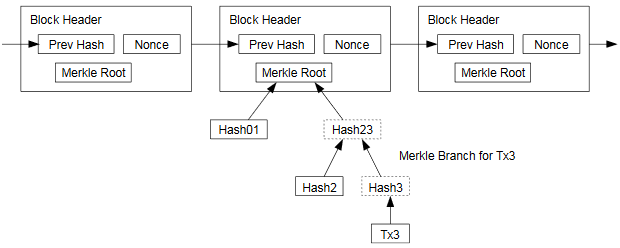
\includegraphics[width=\linewidth]{blockchain}
    \caption{Struttura di una blockchain.}
    \label{fig:blockchain}
\end{figure}

Una \textbf{blockchain} è una architettura di calcolo distribuito funzionante come un registro elettronico senza intermediari
che garantisce l’immutabilità e la permanenza delle informazioni salvate su di essa.

Come suggerisce il nome, la blockchain è una catena di blocchi marcati temporalmente sempre crescente,
nella quale ogni blocco contiene queste informazioni:

\begin{itemize}
    \item Un insieme di transazioni salvate in un Merkle Tree (un albero binario crittograficamente verificato)
    \item L'hash del blocco precedente (nel caso di Ethereum e Bitcoin viene utilizzato l'algoritmo di hashing SHA-256)
    \item Il momento in cui il blocco è stato aggiunto alla catena (sottoforma di timestamp UNIX)
    \item Un nonce, ovvero un numero unico che, inserito in una funzione di hash assieme al resto delle informazioni del blocco,
    permette di ottenere un hash del blocco che è valido se è numericamente inferiore al numero che rappresenta la difficoltà
    della rete.
\end{itemize}

La sicurezza della blockchain è data dalle garanzie delle funzioni di hash: dato che l'header di ogni blocco contiene
l'hash del blocco precedente, se un qualsiasi blocco venisse modificato, il suo hash cambierebbe, e quindi invaliderebbe 
il collegamente al blocco successivo. Bisognerebbe quindi andare a ricalcolare l'hash di ogni blocco successivo,
ma data la dimensione attuale di una blockchain come Bitcoin e la difficoltà della rete
ciò sarebbe computazionalmente quasi impossibile.

La blockchain è nata con Bitcoin, sistema peer-to-peer per una valuta digitale 
ideato da Satoshi Nakamoto nel 2008 basato su una blockchain distribuita e decentralizzata. \cite{ARTICLE:3}
Distribuzione e decentralizzazione sono fondamentali perché rendono la blockchain di fatto incensurabile
e senza un unico point-of-failure. Chiunque può unirsi alla rete Bitcoin: è sufficiente eseguire un client
Bitcoin che gestisce un wallet (una chiave privata, una chiave pubblica ed un indirizzo Bitcoin) 
e connette il dispositivo su cui è installato come nodo della rete.

\subsection{Transazioni}

Lo scambio di valore (e opzionalmente dati) tra due account in una blockchain avviene tramite una \textbf{transazione}. 
Una transazione è un messaggio inviato dall'indirizzo mittente alla blockchain contenente un indirizzo destinatario, il valore della transazione
(anche 0), un nonce (solo per Ethereum, un numero unico per account incrementale per evitare il doppio invio di transazioni), un campo dati
(anche vuoto) e le tre componenti di una firma ECDSA \emph{r}, \emph{s} e \emph{v}.

Una volta inviata, la transazione entra in un \emph{transaction pool}, da dove i miner andranno a selezionare randomicamente transazioni 
da includere nel prossimo blocco. Una transazione che viene correttamente inclusa in un blocco è definitiva e irreversibile.

\subsection{Algoritmi di consenso}

Affinché tutti i nodi partecipanti ad una rete come Bitcoin raggiungano un accordo su quale sarà il prossimo blocco da aggiungere alla blockchain
e quindi ottenere un unico stato del registro elettronico condiviso è necessario implementare un \textbf{algoritmo di consenso}.

\subsubsection{Proof of Work}

Nel caso di Bitcoin ed Ethereum l'algoritmo utilizzato è \textbf{Proof of Work}: per raggiungere consenso sullo stato della blockchain Proof of Work
(in breve PoW) si avvale di particolari nodi chiamati \emph{miner}. I miner prendono delle transazioni dal \emph{transaction pool} e le inseriscono
in un blocco: affinché questo venga accettato dal resto della rete e aggiunto alla blockchain un miner deve trovare un \emph{nonce},
ovvero un numero che, se inserito in una funzione di hash assieme al contenuto del blocco, permette di ottenere un hash numericamente minore
della difficoltà della rete. Questo calcolo, essendo computazionalmente molto costoso, permette di evitare lo spam di blocchi sulla rete, ma essendo
anche economicamente parecchio oneroso a causa della grande quantità di elettricità usata nel calcolo dell'hash corretto, è necessario garantire un incentivo
economico ai miner che aggiungono con successo un blocco alla blockchain: da qui nascono le criptovalute. Quando un blocco viene aggiunto
alla blockchain il miner che l'ha sottoposto allo scrutinio del resto dei nodi che l'hanno validato e approvato viene ricompensato con della
criptovaluta (Ad oggi un miner su Bitcoin viene ricompensato con 12,5 BTC a blocco e 5 Ether a blocco su Ethereum).
Il Proof of Work ha però dei problemi, principalmente due: l'enorme impatto ambientale a causa della grande quantità
di energia elettrica utilizzata dai miner e la centralizzazione della potenza di hashing causata dalla creazione
di potenti gilde di miner che stanno monopolizzando sia la rete Bitcoin che quella Ethereum.

\subsubsection{Proof of Stake}

A causa degli svantaggi sopra elencati di Proof of Work si stanno ricercando algoritmi di consenso alternativi
che vadano ad eliminare (o almeno a ridurre drasticamente) i problemi che lo affliggono. 

L'algoritmo che molto probabilmente andrà a sostituire PoW è \textbf{Proof of Stake} (in breve PoS).
In Proof of Stake i miner vengono sostuituiti dai \emph{validatori}, i quali hanno lo stesso compito dei primi,
ovvero quello di validare transazioni ed inserirle in un blocco aggiunto alla blockchain.
La differenza sta nel modo in cui vengono selezionati i validatori: se prima più potenza di calcolo
significava pià probabilità di aggiungere un blocco, ora è la quantità di criptovaluta congelata (lo stake) in uno
smart contract a definire la probabilità di validare un blocco ed aggiungerlo alla blockchain.
Con PoS diventa ancora più difficile inserire transazioni fraudolente nella blockchain: con PoW il nodo
maligno prova ad inserire transazioni fasulle al massimo perde tempo, con PoS perde direttamente la criptovaluta
congelata sullo smart contract.
PoS va a ridurre drasticamente sia l'impatto ambientale, dato che non serve particolare potenza di calcolo per validare
i blocchi, sia il rischio di centralizzazione, cosa che può sembrare controintutiva dato che più si mette
criptovaluta nello stake e più si ha probabilità di essere selezionati per validare un blocco. 
Questo vantaggio è dato dalla minore rilevanza delle \textbf{economie di scala}: 
\$10 milioni di criptovaluta daranno esattamente ritorni 10 volte migliori di \$1 milione di criptovaluta,
senza altri guadagni aggiuntivi che invece si hanno quando si va a comprare in massa hardware per milioni di dollari
di qualità maggiore rispetto alla media. \cite{WEBSITE:8}

Ethereum sta implementando Proof of Stake tramite il suo progetto Casper.\footnote{Casper: https://github.com/ethereum/casper}

\section{La blockchain Ethereum}

Ethereum\footnote{Ethereum: https://ethereum.org/} prende tutte le caratteristiche di Bitcoin e le amplia, a partire 
dalla criptovaluta nativa del sistema, l'\emph{Ether}.

L'Ether ha una serie di multipli e sottomultipli, tra cui il più utilizzato in ambito \emph{smart contract} \textbf{wei},
che vale $10^{-18}$ Ether.

L'Ether, oltre a fungere da scambio di valore tra un utente della rete ed un altro, serve anche a pagare il \emph{gas}, ovvero la tassa
introdotta per evitare lo spam di transazioni sulla rete e necessaria per inviare transazioni che possono anche non avere valore,
ma possono ad esempio contenere del codice.

\subsection{Smart contract}

Ethereum infatti rende la sua blockchain facilmente programmabile tramite \textbf{smart contract}, ovvero programmi scritti
in un linguaggio di programmazione ad alto livello come Solidity (simil-JavaScript) o Vyper (simil-Python),
compilati in bytecode e distribuiti sulla blockchain tramite speciali transazioni inviate ad un generico indirizzo \texttt{0x0}. 
Gli smart contract sono eseguiti in un ambiente isolato ed indipendente (e quindi più sicuro)
chiamato \textbf{Smart Contract Execution Engine}, che nel caso di Ethereum prende il nome di EVM (Ethereum Virtual Machine).
Esattamente come in ogni blockchain distribuita e decentralizzata ogni nodo della rete possiede una copia della blockchain stessa
(e quindi ogni transazione), in Ethereum ogni nodo esegue il codice degli smart contract: questa replicazione rende molto lenta
l’esecuzione delle istruzioni, ma permette lo sviluppo di applicazioni che necessitano di trasparenza, estrema sicurezza ed immutabilità.

\subsection{Solidity: un linguaggio per lo sviluppo di smart contract}

Solidity\footnote{Solidity: https://github.com/ethereum/solidity} è un linguaggio procedurale ad alto livello ispirato a JavaScript
per lo sviluppo di smart contract.
\`E di gran lunga il linguaggio più diffuso e supportato per lo sviluppo di smart contract, ed
è anche quello più maturo.

La sintassi è familiare, ma ha alcune peculiarità derivanti dal fatto che ha a che fare con
transazioni monetarie e non.

\subsubsection{Oggetti globali}

Solidity ha definiti come oggetti globali \texttt{msg}, \texttt{block} e \texttt{tx},
che contengono rispettivamente informazioni riguardo alla chiamata che ha iniziato 
l'esecuzione dello smart contract (come valore della transazione e indirizzo chiamante), al blocco corrente 
(come numero e timestamp del blocco) e alla transazione (come origine della transazione e costo in gas).

\subsubsection{Tipi di dato}

I tipi sono quelli standard, con la particolarità che il tipo \texttt{string} è stato aggiunto solo molto
dopo la creazione del linguaggio e ad ora non ci sono metodi nativi del linguaggio per lavorare sulle stringhe.
Un tipo di dato che è fondamentale in Solidity è \texttt{address}, che ha una serie di proprietà e metodi che
permettono di lavorare su indirizzi Ethereum tra cui:
\begin{itemize}
    \item \texttt{address.balance}: restituisce il bilancio in wei dell'indirizzo
    \item \texttt{address.transfer(wei da inviare)}: invia il dato numero di wei all'indirizzo Ethereum 
    \item \texttt{address.call(payload)}: crea una chiamata di basso livello ad una funzione
\end{itemize}

\subsubsection{Ereditarietà}

Solidity supporta l'ereditarietà tra contratti, permettendo di conseguenza una maggiore modularità del codice andando
però a rendere più difficile l'analisi di contract, motivo per cui sta prendendo molto piede 
Vyper\footnote{Vyper: https://github.com/ethereum/vyper}, il secondo linguaggio più diffuso che ha molti più vincoli sintattici
e non supporta ereditarietà ma è indicato per contesti dove la sicurezza
e la facilità di revisione del codice sono particolarmente importanti.

\subsubsection{Modificatori di funzione}

Un'altra particolarità di Solidity sono i \textbf{modificatori di funzione}, come questo:

\begin{lstlisting}[language=Solidity, numbers=none]
modifier onlyOwner {
    require(msg.sender == owner);
    _;
}
\end{lstlisting}

In particolare questo modificatore permette l'esecuzione della funzione a cui è applicato soltanto se il chiamante
della funzione è il proprietario, ovvero chi l'ha distribuito sulla blockchain o un delegato, dello smart contract.
I modificatori sono infatti molto utili per regolare gli accessi a funzioni, come in questo caso:

\begin{lstlisting}[language=Solidity, numbers=none]
function adminFunction() public onlyOwner {
    // Code accessible only by admin
}
\end{lstlisting}

\subsubsection{Eventi}

Gli eventi sono costrutti Solidity per creare log di transazioni andate a
buon fine e non. Gli eventi sono particolarmente utili per dare un feedback visivo ad un
utente di una dApp sulle'esito di una transazione, in quanto possono essere impostati dei
listener su di essi ed è possibile fare query anche sugli eventi passati.

\subsubsection{Bytecode ed ABI}

Il compilatore \texttt{solc} permette di ottenere l'ABI di uno smart contract ed il bytecode eseguibile dalla EVM
a partire da un codice sorgente in Solidity.
Una \textbf{ABI} (Application Binary Interface) è come un'API a basso livello, funge quindi da interface del contract,
specificando in un formato JSON le funzioni richiamabili con i parametri accettati e le variabili di ritorno.

\subsubsection{Esempio di contract con la rispettiva ABI}

\begin{lstlisting}[language=Solidity, numbers=none]
pragma solidity ^0.4.22;

contract SimpleKeyValue {
  mapping (int => string) keyValueMapping;

  function set (int _key, string _value) public {
    keyValueMapping[_key] = _value;
  }

  function get (int _key) public view returns (string _value) {
    return keyValueMapping[_key];
  }
}
\end{lstlisting}

\begin{lstlisting}[language=JavaScript, numbers=none]
[
    {
        "constant": false,
        "inputs": [
        {
            "name": "_key",
            "type": "int256"
        },
        {
            "name": "_value",
            "type": "string"
        }
        ],
        "name": "set",
        "outputs": [],
        "payable": false,
        "stateMutability": "nonpayable",
        "type": "function"
    },
    {
        "constant": true,
        "inputs": [
        {
            "name": "_key",
            "type": "int256"
        }
        ],
        "name": "get",
        "outputs": [
        {
            "name": "_value",
            "type": "string"
        }
        ],
        "payable": false,
        "stateMutability": "view",
        "type": "function"
    }
]
\end{lstlisting}

\subsection{Perché la blockchain Ethereum per BLINC?}

Oltre a motivi di sicurezza e trasparenza di caricamento e validazione di informazioni
(documenti, certificati, contratti), la blockchain è stata una scelta tecnologica ovvia
per BLINC, in quanto permette di creare una rete di fiducia distribuita e condivisa tra migranti, ACLI e aziende,
nella quale ognuno dei soggetti interessati può partecipare equamente ed avere accesso ad un'informazione trasparente.

Tra tutte le possibili alternative è stato scelto Ethereum perché, nonostante la giovinezza
del progetto, si è già imposto come standard \emph{de-facto}
per lo sviluppo di applicazioni decentralizzate basate su smart contract
(è stato il primo a portare il concetto di smart contract su architetture
basate su blockchain, poi è stato seguito da altri progetti come EOS e NEO)
e su un frontend che utilizza librerie come web3.js per comunicare con la rete Ethereum,
è supportato dalla più grande comunità open source in ambito blockchain ed è fornito di
un grande numero di strumenti per velocizzare il workflow di sviluppo di \emph{dApp}
(Decentralized Applications), tra cui Truffle\footnote{Truffle: https://truffleframework.com/}, che facilita e
automatizza task di compilazione e migrazione di contratti su diversi tipi di blockchain, e Ganache
\footnote{Ganache: https://truffleframework.com/ganache}, una simulazione in
JavaScript di una blockchain locale che, in quanto non ha necessità di minare le
transazioni, è molto veloce e quindi adatta allo sviluppo e al testing di smart contract.

Essendo quindi un sistema stabile, ben supportato e facilmente integrabile con metodi di sviluppo 
tradizionali grazie alle librerie in JavaScript costantemente aggiornate, 
Ethereum permette di rendere BLINC, oltre che a un progetto di ricerca, un prodotto vendibile.